Mexico City is built in a beautiful valley known as the Valley of Mexico which, years ago, was mostly a lake. Around the year 1300, Aztec religious leaders decreed that the lake's center be filled in order to build the capital of their empire. Today, the lake is completely covered.

Before the Aztecs arrived, c cities were located around the lake on its shores. Some of these cities established commercial agreements. Goods were traded, using boats, between cities that had a commercial agreement. It was possible to connect any two cities by a line segment through the lake.

Eventually, the kings of the cities decided to organize this commerce. They designed a commerce route that connected every city around the lake. The route met the following requirements:
\begin{itemize}
\item It could start in any of the cities, visited each of the cities around the lake, and finally endedin another city different from the starting city.
\item The route visited each city exactly once.
\item Every pair of consecutively visited cities in the route had a commercial agreement.
\item Every pair of consecutively visited cities in the route was connected by a line segment.
\item To avoid crashes between boats, the route never crossed itself.
\end{itemize}

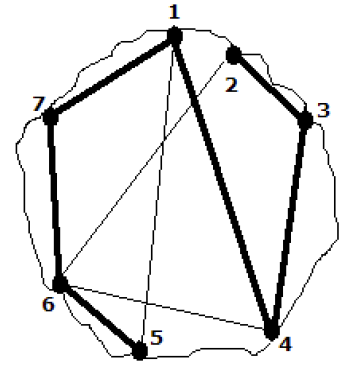
\includegraphics{mexico.png}

The figure shows the lake and the cities around it. The lines (both thick and thin) represent commercial agreements between cities. The thick lines represent a
commerce route starting in city 2 and ending in city 5.

This route never crosses itself. It would not be legal, for example, to construct a route that went from 2 to 6 to 5 to 1, since the route would cross itself.

Cities in the lake are numbered from 1 through $c$ moving in clockwise direction.

Write a program that, given both the count $c$ of cities and a list of the commercial agreements between them, constructs a commerce route that meets the above requirements.